\documentclass[12pt, twoside]{article}
\usepackage{jmlda}
\newcommand{\hdir}{.}

% notations
% bold
\newcommand{\ba}{\mathbf{a}}
\newcommand{\bz}{\mathbf{z}}
\newcommand{\bx}{\mathbf{x}}
\newcommand{\by}{\mathbf{y}}
\newcommand{\bw}{\mathbf{w}}
\newcommand{\bfx}{\mathbf{f}}
\newcommand{\bb}{\mathbf{b}}
\newcommand{\bu}{\mathbf{u}}
\newcommand{\bX}{\mathbf{X}}
\newcommand{\bZ}{\mathbf{Z}}
\newcommand{\bA}{\mathbf{A}}
\newcommand{\bB}{\mathbb{B}}
\newcommand{\bI}{\mathbf{I}}
\newcommand{\bJ}{\mathcal{J}}
\newcommand{\bV}{\mathbf{V}}
\newcommand{\bU}{\mathbf{U}}
\newcommand{\bG}{\mathbf{G}}
\newcommand{\bQ}{\mathbf{Q}}
\newcommand{\bchi}{\mathbf{\chi}}
\newcommand{\btheta}{\boldsymbol{\theta}}
\newcommand{\bPsi}{\boldsymbol{\Psi}}
\newcommand{\bpsi}{\boldsymbol{\psi}}
\newcommand{\bxi}{\boldsymbol{\xi}}
\newcommand{\bzeta}{\boldsymbol{\zeta}}
\newcommand{\blambda}{\boldsymbol{\lambda}}
\newcommand{\beps}{\boldsymbol{\varepsilon}}
\newcommand{\bZeta}{\boldsymbol{Z}}
% mathcal
\newcommand{\cX}{\mathcal{X}}
\newcommand{\cY}{\mathcal{Y}}
\newcommand{\cW}{\mathcal{W}}
\newcommand{\cN}{\mathcal{N}}
\newcommand{\cD}{\mathcal{D}}
% transpose
\newcommand{\getT}{^{\mathsf{T}}}


\begin{document}

\title
    [Байесовский выбор структур обобщенно-линейных моделей] % краткое название; не нужно, если полное название влезает в~колонтитул
    {Байесовский выбор структур обобщенно-линейных моделей}
\author
    [A.\,Д.~Толмачев] % список авторов (не более трех) для колонтитула; не нужен, если основной список влезает в колонтитул
    {A.\,Д.~Толмачев, А.\,А.~Адуенко, В.\,В.~Стрижов} % основной список авторов, выводимый в оглавление
    [А.\,Д.~Толмачев, А.\,А.~Адуенко, В.\,В.~Стрижов] % список авторов, выводимый в заголовок; не нужен, если он не отличается от основного
\email
    {tolmachev.a.d.@phystech.edu; aduenko1@gmail.com; strijov@ccas.ru}
\thanks
    {Работа выполнена в рамках курса <<Моя первая научная статья>>, НИУ МФТИ, 2021}
    
\abstract
    {В данной работе исследуется проблема мультиколлинеарности и её влияние
    на точность методов выбора признаков. Решается задача выбора признаков и различные подходы к ее решению. Исследовано применение байесовского подхода для метода отбора признаков на основе квадратичного программирования. В работе приводятся критерии сравнения различных способов отбора признаков, и проведено сравнение различных методов на тестовых выборках.
    Сделан вывод об эффективности рассматриваемых подходов на синтетических данных.

\bigskip
\noindent
\textbf{Ключевые слова}: \emph {регрессионный анализ; мультиколлинеарность; байесовский подход; выбор признаков;  квадратичное программирование}
}

%данные поля заполняются редакцией журнала
%\doi{}
%\receivedRus{}
%\receivedEng{}

\maketitle
\linenumbers

\section{Введение}
Работа посвящена анализу применения байесовского подхода для методов отбора признаков и сравнительному анализу различных методов отбора признаков. Предполагается, что исследуемая выборка содержит значительное число мультиколлинеарных признаков. Мультиколлинеарность — это сильная корреляционная связь между отбираемыми для анализа признаками, совместно
воздействующими на целевой вектор. Это явление затрудняет оценивание регрессионных параметров и выявление зависимости между признаками и целевым вектором. Проблема мультиколлинеарности и возможные способы её обнаружения и устранения описаны в \cite{SneeRon, Leamer, Askin}. 

Задача выбора оптимального подмножества признаков является одной из основных частей выбора модели в исследуемом методе обучения (см. в \cite{Bolon-Canedo}).
Методы выбора признаков основаны на минимизации некоторого функционала, который отражает качество
рассматриваемого подмножества признаков. В \cite{FeatureSelection1, FeatureSelection2} сделан обзор основных существующих методов отбора признаков.

В \cite{KatrutsaS17} предложен новый метод отбора признаков, использующий один из основных методов оптимизации, квадратичное программирование (см. \cite{Rodriguez}), для задачи отбора признаков. Цель данной работы состоит в анализе возможностей применения байесовского подхода для метода квадратичного программирования в задаче выбора признаков. 

Важной частью этой работы является сравнение метода на основе байесовского подхода и других методов отбора признаков, описанных, например, в \cite{Katrutsa15}, на различных тестовых выборках.


\section{Постановка задачи}

\subsection{Рассматриваемая модель}
Задана выборка $\mathcal{D} = \{(\bx_i, y_i)\}$, где $i \in \{1, 2, ..., m\}$, где множество свободных переменных --- вектор $\bx = [x_1, x_2, ...,x_j, ..., x_n]$, где $j \in \bJ = \{1, 2, ...., n\}$. Предполагается, что $\bx_i \in \mathbb{X} \subset \mathbb{R}^n$ и $y_i \in \mathbb{Y} \subset \mathbb{R}$.

Введем обозначения $\by = [y_1, y_2, ... y_m]\getT$ - вектор значений зависимой переменной (целевой вектор), $\bchi_j = [x_{1j}, x_{2j}, ..., x_{mj}]\getT$ - реализация $j$-ой свободной переменной ($j$-ый признак), и $\bX = [x_1\getT, x_2\getT, ...x_n\getT]\getT = [\bchi_1, \bchi_2, ..., \bchi_n]$ - матрица плана эксперимента. 

Предполагается, что вектор $\bx_i$ и значение целевой переменной $y_i$ связаны соотношением 

$$y_i = f(\bw, \bx_i) + \varepsilon(\bx_i),$$

где $f: \mathbb{W} \times \mathbb{X} \rightarrow \mathbb{Y}$  есть отображение декартова произведения пространства допустимых параметров $\mathbb{W}$ и пространства значений $\mathbb{X}$ свободной переменной в область значений $\mathbb{Y}$ зависимой целевой переменной, а $\varepsilon(\bx_i)$ - $i$-ый компонент вектора регрессионных остатков $\beps = \bfx - \by.$ Обозначим вектор-функцию $$\bfx = \bfx(\bw, \bX) = [f(\bw, \bx_1), f(\bw, \bx_2), ..., f(\bw, \bx_m)]\getT \in \mathbb{Y}^m.$$

Назовем моделью пару $(\bfx, \mathcal{A})$, где $\mathcal{A} \subset \bJ$ --- подмножество индексов признаков, используемое для вычисления вектор-функции $\bfx$.

На первом уровне байесовского вывода будем задавать априорное распределение на $\beps$ как многомерное нормальное распределение $\mathcal{N}(0, \sigma^2 \mathbf{I}_m).$

\subsection{Применение квадратичной оптимизации для задачи отбора признаков}

В \cite{KatrutsaS17} предлагается подход с применением квадратичной оптимизации для задачи выбора признаков в сформулированной выше модели. Основная идея предлагаемого подхода заключается в минимизации количества схожих признаков и максимизации количества релевантных признаков.
Пусть $\bJ$ -- множество признаков в рассматриваемой модели, и $|\bJ| = n$. 
Зададим функционал $Q(\ba) = \ba \getT \bQ \ba - \bb \getT \ba$, где $\ba \in \mathbb{R}^n$ и $\bQ \in \mathbb{R}^{n \times n}$ -- матрица схожести признаков, а $\bb \in \mathbb{R}^n$ -- вектор релевантности признаков с целевым вектором.
Матрицу $\bQ$ и вектор $\bb$ будем представлять как функции Sim и Rel соответственно, где Sim: $\bJ \times \bJ \rightarrow [0, 1]$, Rel: $\bJ \rightarrow [0, 1]$. Таким образом, необходимо решить задачу оптимизации: 

$$ \ba^* = \arg \min_{a \in \bB^n} Q(\ba).$$

Важно отметить, что задача целочисленного квадратичного программирования, сформулированная выше, является $\mathbf{NP}$-полной, так как поиск минимума функции $\bQ$ ведется по вершинам булева куба $\bB^n = \{0, 1\}^n$. Поэтому, чтобы можно было применять различные методы выпуклой оптимизации будем искать минимум функции по выпуклой оболочке булева куба Conv$(\bB^n) = [0, 1]^n$. 

Тогда получаем следующую задачу выпуклой оптимизации:
\begin{equation*}
\begin{cases}
   $$ \bz^* = \arg \min_{z \in [0, 1]^n}  \bz \getT \bQ \bz - \bb \getT \bz$$  \\
   $$\|z\|_1 \le 1$$
 \end{cases}
 \end{equation*}

Здесь, $Q$ и $b$ по-прежнему являются матрицей схожести признаков и вектором релевантности признаков соответственно. В данной работе функции Sym и Rel (или, другими словами, матрица $Q$ и вектор $b$ в обозначениях выше) задаются заранее до применения метода на основе сходств между признаками в датасете.

Далее положим, $\tau$ - пороговое значение для отбора признаков в данном методе, т.е. $z_i^* > \tau \Leftrightarrow a_i^* = 1 \Leftrightarrow j \in \mathcal{A}$, где $\mathcal{A} \subset \bJ$ -- множество отобранных методом признаков.

Далее предлагается рассмотреть возможные применения байесовского подхода к данному методу квадратичного программирования. Кроме того планируется рассмотреть распределение на $\ba$ как второй уровень байесовского вывода (будет более подробно описано после обсуждения с консультантом).


\subsection{Данные для экспериментов}

В качестве данных для экспериментов по проверке предложенных подходов мы используем синтетические наборы данных из работы \cite{Katrutsa15}, в которых рассматриваются различные типы зависимости признаков между собой и с целевым вектором. Кроме того, будут проведены эксперименты и на ссобственных генерированных синтетических данных.


\section{Базовый эксперимент}

\subsection{Цель}

Как сказано в \cite{KatrutsaS17} метод квадратичного программирования улучшает качество отбора признаков для многих типов выборок. Однако, не во всех случаях этот метод дает наилучшие результаты. Цель базового эксперимента заключается в поиске и рассмотрении выборок с мультиколлинеарными признаками, на которых методу квадратичного программирования не удается провести качественный отбор признаков. Далее планируется исследовать, в чем сходство выборок, на которых метод квадратичного программирования дает неоптимальные результаты, чтобы учесть полученные закономерности при разработке нового метода отбора признаков на основе байесовского подхода.

\subsection{Описание данных}

В качестве базового эксперимента рассмотрим синтетические данные и применим на них метод квадратичного программирования QBFS, описанный выше, для поиска значения $\ba^*$, при котором значение функционала $Q(\ba)$ принимает наименьшее значение.

Рассмотрим модель, в которой будут два признака $x_1, x_2$ и целевая переменная $y$. Пусть $x_1 \sim \cN(0, 1)$, $y \sim \cN(0, 1)$, а $x_2 = x_1 + \beps \cdot y$, т.е. $x_1$ и $y$ - независимые случайные величины из стандартного нормального распределения, а $\varepsilon$ - заранее выбранное малое значение. Таким образом, мы получаем, что $y = \frac{x_2 - x_1}{\beps}$, т.е. целевая переменная зависит от двух признаков. В базовом эксперименте будем генировать при заданном значении $\beps$ выборки объектов и значения целевой переменной, как было описано выше.  Затем получим матрицы $\bQ$ и вектора $\bb$ с помощью нахождения соответствующих коэффициентов корреляции Пирсона. И после этого на получившемся наборе данных будем применять метод квадратичного программирования для поиска оптимального значения двумерного (т.к. в нашей модели два признака) $\ba^*$ в поставленной выше задачи оптимизации.

\subsection{Результаты эксперимента}

Положим $\beps = 0.001$ в обозначениях выше. И будем генерировать выборки размера 1000. Повторим эксперимент несколько раз и посмотрим на получившиеся значения вектора $\ba^* = (a_1, a_2)$ в каждом из случаев. Так как $\ba^* \in [0, 1]^2$ согласно поcтановке нашей задачи и значения компонент вектора $\ba^*$ могут принимать малые значения, то построим график логарифмов этих коэффициентов. 

\begin{figure}[htb]
\center{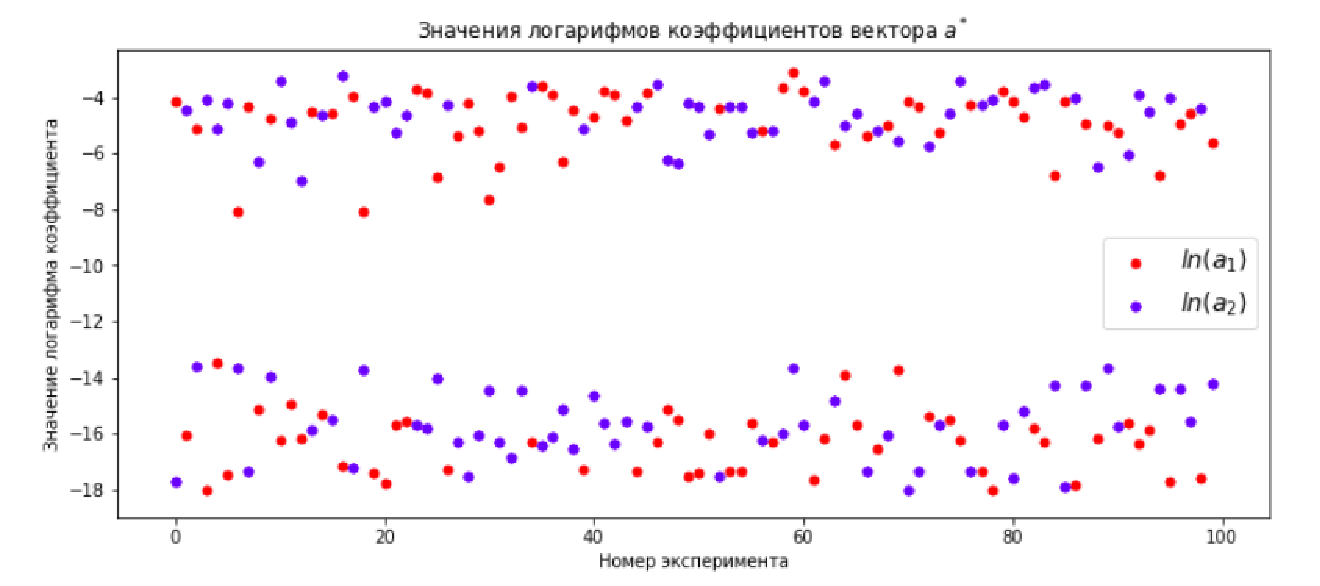
\includegraphics[width=17cm]{base_exp.pdf}}
\caption{результаты базового эксперимента}
\label{fig:image, d11_lower_pic}
\end{figure}


Было проведено 100 экспериментов, в каждом из которых был найден вектор $\ba^*$. Как можно видеть по графику, метод квадратичного программирования отбирает в каждом случае только один из признаков, т.к. мы видим на графике, что значения логарифмов отличатся, а значит, значения самих компонент $a_1$ и $a_2$ отличаются на несколько порядков. Таким образом, мы получили, что в данном эксперименте метод квадратичного программирования отбирает только один признак, причем примерно в половине экспериментов отбирается первый признак, и примерно в половине - второй признак. Т.е. нельзя сказать, что один из признаков в данном случае наиболее значим и было бы лучше, чтобы метод отбирал оба признака.



\section{Название раздела}
Данный документ демонстрирует оформление статьи,
подаваемой в электронную систему подачи статей \url{http://jmlda.org/papers} для публикации в журнале <<Машинное обучение и анализ данных>>.
Более подробные инструкции по~стилевому файлу \texttt{jmlda.sty} и~использованию издательской системы \LaTeXe\
находятся в~документе \texttt{authors-guide.pdf}.
Работу над статьёй удобно начинать с~правки \TeX-файла данного документа.

Обращаем внимание, что данный документ должен быть сохранен в кодировке~\verb'UTF-8 without BOM'.
Для смены кодировки рекомендуется пользоваться текстовыми редакторами \verb'Sublime Text' или \verb'Notepad++'.

\paragraph{Название параграфа}
Разделы и~параграфы, за исключением списков литературы, нумеруются.

\section{Заключение}
Желательно, чтобы этот раздел был, причём он не~должен дословно повторять аннотацию.
Обычно здесь отмечают, каких результатов удалось добиться, какие проблемы остались открытыми.


\bibliographystyle{plain}
\bibliography{Tolmachev2021BayesApproach.bib}

\end{document}
